\documentclass[
    fontsize=11pt,
    paper=a4,
    parskip=half,
    abstract=on
]{scrartcl}

\usepackage[utf8]{inputenc}
\usepackage[T1]{fontenc}
\usepackage[scaled]{helvet}
\renewcommand{\familydefault}{\sfdefault}
\usepackage{geometry}
\geometry{margin=1in}

\usepackage{hyperref}
\usepackage{url}
\usepackage{graphicx}
\usepackage{xcolor}
\usepackage{tcolorbox}
\usepackage{enumitem}
\usepackage{natbib}
\usepackage{tikz}
\usetikzlibrary{positioning,shapes.geometric,arrows.meta}

% Define Colors
\definecolor{primary}{HTML}{7B4384}
\definecolor{secondary}{HTML}{A577B8}
\definecolor{tertiary}{HTML}{765F93}
\definecolor{accent}{HTML}{DDAEE4}

% Apply to KOMA-Script Elements
\addtokomafont{title}{\color{primary}\bfseries}
\addtokomafont{section}{\color{primary}\sffamily}
\addtokomafont{subsection}{\color{secondary}\sffamily}
\addtokomafont{author}{\color{secondary}\sffamily}
\addtokomafont{date}{\color{tertiary}\sffamily}
\addtokomafont{captionlabel}{\color{tertiary}\bfseries}

% Tool Card Definitions
% Objective box - lightest purple
\newtcolorbox{objectivebox}[2][]{
    colback=accent!25!white,
    colframe=accent!80!primary,
    colbacktitle=accent!80!primary,
    coltitle=white,
    title=\textbf{#2},
    fonttitle=\bfseries\large,
    #1
}

% Technical requirements box - medium purple
\newtcolorbox{techbox}[2][]{
    colback=secondary!15!white,
    colframe=secondary!90!black,
    colbacktitle=secondary,
    coltitle=white,
    title=\textbf{#2},
    fonttitle=\bfseries\large,
    #1
}

% Resources box - darker purple
\newtcolorbox{resourcebox}[2][]{
    colback=primary!10!white,
    colframe=primary,
    colbacktitle=tertiary,
    coltitle=white,
    title=\textbf{#2},
    fonttitle=\bfseries\large,
    #1
}

% Legacy toolcard (for compatibility)
\newtcolorbox{toolcard}[2][]{
    colback=accent!15!white,
    colframe=primary,
    colbacktitle=secondary,
    coltitle=white,
    title=\textbf{#2},
    fonttitle=\bfseries\large,
    #1
}

\title{AI Safety Tools and Interpretability Frameworks}
\subtitle{A Comprehensive Technical Reference}
\author{Elisabetta Rocchetti}
\date{\today}

\begin{document}

\maketitle

\begin{abstract}
This document provides a comprehensive survey of tools and frameworks for AI safety research and mechanistic interpretability. The field has rapidly evolved to address the critical need for understanding, evaluating, and controlling the behavior of large language models and other neural networks. The tools covered span three main categories: evaluation frameworks for assessing model capabilities and risks, mechanistic interpretability libraries for understanding model internals through techniques like sparse autoencoders and circuit analysis, and intervention frameworks for causally probing and steering model behavior. Each tool is described with standardized information including capabilities, supported models, computational requirements, and programmatic accessibility. This reference aims to help researchers select appropriate tools for their specific AI safety and interpretability research needs.
\end{abstract}

\section{Introduction}

Understanding and ensuring the safety of AI systems has become one of the most pressing technical challenges in machine learning research~\citep{amodei2016concrete}. As models grow in capability and deployment scale, the need for rigorous evaluation, deep interpretability, and precise control mechanisms has intensified. This document catalogs the major open-source tools that enable such research.

The tools described here fall into three broad categories. First, \textbf{evaluation frameworks} provide systematic methods for assessing model capabilities, identifying vulnerabilities, and measuring safety-relevant properties. Second, \textbf{mechanistic interpretability tools} enable researchers to peer inside neural networks, decomposing their computations into interpretable components like features and circuits. Third, \textbf{intervention frameworks} allow researchers to causally probe models by modifying internal activations and observing the effects.

Together, these tools form an ecosystem that supports the technical work necessary to build AI systems that are transparent, controllable, and aligned with human intentions. While no single tool solves all problems, the combination of rigorous evaluation, deep understanding, and precise intervention provides the foundation for safer AI development.

\section{Evaluation Frameworks}

Evaluation frameworks provide structured approaches to assess AI model capabilities, safety properties, and potential risks. Unlike ad-hoc testing, these frameworks offer reproducible, scalable methods for systematic evaluation.

\subsection{Inspect AI}

Inspect is a comprehensive framework for large language model evaluations developed by the UK AI Safety Institute~\citep{inspect2024}. It provides built-in components for prompt engineering, tool usage, multi-turn dialog, and model-graded evaluations, with extensive support for custom evaluation development. The framework supports systematic capability evaluations across multiple models, safety and alignment testing, tool use and agent behavior assessment, and custom evaluation development and benchmarking. Inspect focuses on black-box evaluation rather than inspecting model internals, producing evaluation results, metrics, logs, and detailed HTML reports with visualization.

\begin{objectivebox}{Objective \& Scope}
\textbf{Primary Purpose:} Framework for systematic LLM capability and safety evaluation through reproducible benchmarks.

\textbf{Scope:} Black-box evaluation (no model internals access), API and local models, custom evaluation development, multi-model comparisons.

\textbf{Output:} Evaluation metrics, performance reports, HTML visualizations, detailed logs.
\end{objectivebox}

\begin{techbox}{Technical Requirements}
\textbf{Supported Models:} Any LLM accessible via API (OpenAI, Anthropic, Together, etc.) or locally via HuggingFace.

\textbf{Compute Requirements:} Minimal for framework; depends on models being evaluated. Can run on standard laptop for API-based models.

\textbf{Dependencies:} Python 3.10+, PyTorch (optional for local models).

\textbf{Usage:} Programmatic Python library with CLI interface. Can be integrated into CI/CD pipelines.
\end{techbox}

\begin{resourcebox}{Resources}
\textbf{Repository:} \url{https://github.com/UKGovernmentBEIS/inspect_ai}

\textbf{Documentation:} \url{https://inspect.aisi.org.uk/}

\textbf{Key Features:} Extensible solver and scorer system; built-in support for tool calling; dataset integration; parallel execution; detailed logging.
\end{resourcebox}

\subsection{Inspect Evals}

A collection of over 100 pre-built evaluations that work with the Inspect AI framework~\citep{inspectevals2024}. Covers diverse areas including knowledge (MMLU, TruthfulQA, SciQ), reasoning (GSM8K, MATH, ARC), safety (ToxiGen, BOLD, BBQ bias benchmarks), agent capabilities (WebArena, SWE-bench), and security (CyberSecEval, secure code generation). This evaluation-focused toolkit produces standardized evaluation metrics and comparison reports without requiring access to model internals.

\begin{objectivebox}{Objective \& Scope}
\textbf{Primary Purpose:} Ready-to-use evaluation suite covering knowledge, reasoning, safety, and agent capabilities.

\textbf{Scope:} 100+ pre-built benchmarks, standardized metrics, works with Inspect AI framework.

\textbf{Output:} Benchmark scores, comparison reports, standardized evaluation results.
\end{objectivebox}

\begin{techbox}{Technical Requirements}
\textbf{Supported Models:} Same as Inspect AI (any API or local LLM).

\textbf{Compute Requirements:} Varies by evaluation; most run efficiently on standard hardware.

\textbf{Dependencies:} Requires Inspect AI framework.

\textbf{Usage:} Programmatic library; evaluations can be run individually or in batches.
\end{techbox}

\begin{resourcebox}{Resources}
\textbf{Repository:} \url{https://github.com/UKGovernmentBEIS/inspect_evals}

\textbf{Documentation:} \url{https://ukgovernmentbeis.github.io/inspect_evals/}
\end{resourcebox}

\subsection{ControlArena}

A framework for evaluating AI control protocols and oversight mechanisms~\citep{controlarena2024}. Tests how well monitoring systems can detect and prevent undesired model behaviors, supporting testing of AI control and monitoring strategies, evaluating red-teaming effectiveness, measuring detectability of deceptive behaviors, and oversight protocol development. The framework provides limited intervention support, focusing primarily on behavioral evaluation under different control regimes, and produces control effectiveness metrics, detection rates, and protocol performance analysis.

\begin{objectivebox}{Objective \& Scope}
\textbf{Primary Purpose:} Evaluate AI control protocols and oversight mechanisms for detecting/preventing undesired behaviors.

\textbf{Scope:} Red-team/blue-team scenarios, monitoring strategy testing, deception detection, limited intervention support.

\textbf{Output:} Control effectiveness metrics, detection rates, protocol performance analysis.
\end{objectivebox}

\begin{techbox}{Technical Requirements}
\textbf{Supported Models:} LLMs accessible via standard APIs.

\textbf{Compute Requirements:} Moderate; requires running multiple model instances for red-team/blue-team scenarios.

\textbf{Dependencies:} Python, Inspect AI framework.

\textbf{Usage:} Programmatic interface for defining control protocols and evaluation scenarios.
\end{techbox}

\begin{resourcebox}{Resources}
\textbf{Repository:} \url{https://github.com/UKGovernmentBEIS/control-arena}
\end{resourcebox}

\section{Mechanistic Interpretability Tools}

Mechanistic interpretability aims to reverse-engineer neural networks by identifying the algorithms and representations they learn~\citep{olah2020zoom}. These tools enable researchers to decompose model computations into interpretable components.

\subsection{TransformerLens}

A library specifically designed for mechanistic interpretability of GPT-style language models~\citep{transformerlens2024}. Provides easy access to all model internals with clean, interpretable activations and comprehensive hooks for activation caching and analysis, circuit discovery and tracing, attention pattern visualization, studying induction heads and algorithmic circuits, and feature attribution and ablation studies. The library offers comprehensive support for activation patching, ablations, and causal interventions at any layer or component. Outputs include tensors of activations, attention patterns, and logits, with integration to CircuitsVis for visualization.

\begin{objectivebox}{Objective \& Scope}
\textbf{Primary Purpose:} Full-featured library for mechanistic interpretability of transformer language models.

\textbf{Scope:} Complete activation access, circuit discovery, attention analysis, intervention support (patching/ablations).

\textbf{Output:} Activation tensors, attention patterns, logits, visualizations via CircuitsVis.
\end{objectivebox}

\begin{techbox}{Technical Requirements}
\textbf{Supported Models:} GPT-2, GPT-Neo, GPT-J, Pythia, OPT, BLOOM, LLaMA family, Gemma, Mistral; dozens of pre-configured models.

\textbf{Compute Requirements:} Moderate to high; requires loading full model weights. GPU recommended for models larger than 1B parameters.

\textbf{Dependencies:} PyTorch, transformers, einops, fancy\_einsum.

\textbf{Usage:} Programmatic Python library; designed for notebook-based exploratory analysis. Extensive tutorial notebooks available.
\end{techbox}

\begin{resourcebox}{Resources}
\textbf{Repository:} \url{https://github.com/TransformerLensOrg/TransformerLens}

\textbf{Documentation:} \url{https://transformerlensorg.github.io/TransformerLens/}

\textbf{Key Features:} Clean, factored activation access; modular intervention system; caching for efficient experimentation; extensive model zoo.
\end{resourcebox}

\subsection{CircuitTracer}

A library for finding circuits using features from cross-layer MLP transcoders~\citep{circuittracer2025}. Implements the attribution graph methods introduced by Anthropic's circuit discovery research, computing direct effects between transcoder features, error nodes, tokens, and output logits. Enables circuit discovery using transcoder features, attribution graph computation and visualization, feature-level intervention experiments, integration with Neuronpedia for graph exploration, and support for both programmatic and CLI-based workflows. Works with pre-trained transcoders (PLTs and CLTs) for Gemma-2, Llama-3.2, and Qwen-3 models, producing attribution graphs, interactive visualizations, and intervention results.

\begin{objectivebox}{Objective \& Scope}
\textbf{Primary Purpose:} Find circuits using transcoder features via attribution graphs; compute direct effects between features, tokens, and logits.

\textbf{Scope:} Attribution graph computation, circuit visualization, feature interventions, Neuronpedia integration, supports TransformerLens/nnsight backends.

\textbf{Output:} Attribution graphs, interactive visualizations (web-based), intervention results, graph annotations.
\end{objectivebox}

\begin{techbox}{Technical Requirements}
\textbf{Supported Models:} Gemma-2 (2B), Llama-3.2 (1B), Qwen-3 (0.6B-14B); requires pre-trained transcoders. Can use TransformerLens or nnsight backend.

\textbf{Compute Requirements:} Moderate; Gemma-2 2B works on Colab free tier (15GB VRAM). Larger models benefit from more GPU memory to reduce offloading.

\textbf{Dependencies:} PyTorch, transformers, TransformerLens (default) or nnsight (experimental backend).

\textbf{Usage:} Python library (Jupyter notebooks/scripts) or CLI. Integrates with Neuronpedia web interface for visualization.
\end{techbox}

\begin{resourcebox}{Resources}
\textbf{Repository:} \url{https://github.com/safety-research/circuit-tracer}

\textbf{Documentation:} Tutorial notebooks available; see \url{https://transformer-circuits.pub/2025/attribution-graphs/methods.html}

\textbf{Key Features:} Transcoder-based attribution graphs; interactive visualization server; Neuronpedia integration; feature intervention capabilities; CLI workflow; supports PLTs and CLTs.
\end{resourcebox}

\subsection{nnsight}

A framework for interpreting and intervening on the internals of PyTorch models~\citep{nnsight2024}. Provides a unified interface for accessing activations, performing interventions, and tracing computations. Enables remote model access via NDIF (National Deep Inference Fabric), distributed interpretability research, activation extraction and intervention, and cross-model comparison studies. Offers full support for intervention on any module's inputs and outputs, producing PyTorch tensors, intervention results, and computation traces.

\begin{objectivebox}{Objective \& Scope}
\textbf{Primary Purpose:} Unified framework for interpreting PyTorch models with remote compute access via NDIF.

\textbf{Scope:} Model-agnostic activation access, full intervention support, distributed research, local/remote execution.

\textbf{Output:} PyTorch tensors, intervention results, computation traces.
\end{objectivebox}

\begin{techbox}{Technical Requirements}
\textbf{Supported Models:} Any PyTorch model; strong support for HuggingFace models.

\textbf{Compute Requirements:} Variable; can use remote compute via NDIF for expensive operations.

\textbf{Dependencies:} PyTorch, transformers.

\textbf{Usage:} Programmatic Python library with both local and remote execution modes.
\end{techbox}

\begin{resourcebox}{Resources}
\textbf{Repository:} \url{https://github.com/ndif-team/nnsight}

\textbf{Documentation:} \url{https://nnsight.net/}

\textbf{Key Features:} Remote model access; unified API across architectures; efficient batched interventions; grad-compatible operations.
\end{resourcebox}

\subsection{SAELens}

A comprehensive library for training and analyzing Sparse Autoencoders (SAEs) on language models~\citep{saelens2024}. SAEs decompose neural network activations into sparse, interpretable features that often correspond to human-understandable concepts~\citep{cunningham2023sparse}. The library supports training SAEs on model activations, loading and analyzing pre-trained SAEs, feature discovery and interpretation, activation reconstruction analysis, and generating feature dashboards. SAE features can be used for targeted interventions and steering, with outputs including trained SAE weights, feature activations, reconstruction statistics, and visualization dashboards. An extensive collection of pre-trained SAEs for GPT-2, Pythia, Gemma, and other models is available via HuggingFace.

\begin{objectivebox}{Objective \& Scope}
\textbf{Primary Purpose:} Train and analyze Sparse Autoencoders to decompose model activations into interpretable features.

\textbf{Scope:} SAE training (multiple architectures), pre-trained SAE library, feature interpretation, intervention via features.

\textbf{Output:} Trained SAE weights, feature activations, reconstruction statistics, visualization dashboards.
\end{objectivebox}

\begin{techbox}{Technical Requirements}
\textbf{Supported Models:} Deep integration with TransformerLens; also works with HuggingFace models, nnsight, and custom PyTorch models via encode/decode methods.

\textbf{Compute Requirements:} High for training (GPU required; training can take hours to days). Moderate for inference.

\textbf{Dependencies:} PyTorch, transformers, TransformerLens (for tight integration), wandb (for training monitoring).

\textbf{Usage:} Programmatic Python library. Training via config files or Python API; analysis via notebooks.
\end{techbox}

\begin{resourcebox}{Resources}
\textbf{Repository:} \url{https://github.com/jbloomAus/SAELens}

\textbf{Documentation:} \url{https://jbloomaus.github.io/SAELens/}

\textbf{Key Features:} Multiple SAE variants (vanilla, TopK, Gated); pre-trained SAE library; automated interpretability via GPT-4; integration with SAE-Vis for dashboards; supports distributed training.
\end{resourcebox}

\subsection{Neuronpedia}

An open platform for sharing and exploring interpretability artifacts, particularly SAE features and circuits~\citep{neuronpedia2024}. Functions as a collaborative database and visualization tool for mechanistic interpretability research, enabling browsing of pre-computed SAE features, visualizing feature activations and examples, sharing interpretability findings, exploring circuits and computational graphs, and community collaboration on feature interpretation. This primarily visualization and exploration platform produces interactive web visualizations, feature dashboards, and circuit diagrams, with no computational requirements for users as it is entirely web-based.

\begin{objectivebox}{Objective \& Scope}
\textbf{Primary Purpose:} Collaborative web platform for exploring and sharing SAE features and interpretability findings.

\textbf{Scope:} Web-based visualization, pre-computed feature database, community annotations, circuit exploration.

\textbf{Output:} Interactive web visualizations, feature dashboards, circuit diagrams.
\end{objectivebox}

\begin{techbox}{Technical Requirements}
\textbf{Supported Models:} GPT-2, Claude Sonnet (via Anthropic's public SAEs), Gemma; expanding coverage.

\textbf{Compute Requirements:} None for users (web-based platform).

\textbf{Dependencies:} Web browser for access; Python API available for programmatic upload/download of features.

\textbf{Usage:} Web application for browsing; Python API for programmatic interaction.
\end{techbox}

\begin{resourcebox}{Resources}
\textbf{Website:} \url{https://neuronpedia.org/}

\textbf{Repository:} \url{https://github.com/hijohnnylin/neuronpedia}

\textbf{Key Features:} Large database of interpreted features; community annotations; circuit visualization; integration with SAELens and Anthropic's work; search and filter capabilities.
\end{resourcebox}

\subsection{CircuitsVis}

A library of React-based visualizations for mechanistic interpretability~\citep{circuitsvis2024}. Works seamlessly in both Python (Jupyter) and JavaScript environments for attention pattern visualization, token-level attribution display, neuron activation heatmaps, logit lens visualizations, and interactive exploration of model internals. This visualization-focused tool produces interactive HTML visualizations renderable in notebooks or web pages, requiring minimal compute for lightweight visualization rendering.

\begin{objectivebox}{Objective \& Scope}
\textbf{Primary Purpose:} React-based visualization library for attention patterns, activations, and interpretability artifacts.

\textbf{Scope:} Model-agnostic, works in Python (Jupyter) and JavaScript, interactive HTML visualizations.

\textbf{Output:} Interactive HTML visualizations for notebooks/web pages.
\end{objectivebox}

\begin{techbox}{Technical Requirements}
\textbf{Supported Models:} Model-agnostic (works with any activation data).

\textbf{Compute Requirements:} Minimal (lightweight visualization rendering).

\textbf{Dependencies:} React (for JS usage); ipython for Python usage.

\textbf{Usage:} Dual-use library with Python functions for notebooks and React components for web integration.
\end{techbox}

\begin{resourcebox}{Resources}
\textbf{Repository:} \url{https://github.com/TransformerLensOrg/CircuitsVis}

\textbf{Documentation:} \url{https://transformerlensorg.github.io/CircuitsVis/}

\textbf{Key Features:} Attention head visualization; token-based coloring; logit lens; neuron activation displays; works offline; customizable styling.
\end{resourcebox}

\subsection{Transformer Debugger (TDB)}

An interactive tool developed by OpenAI for investigating specific behaviors in small language models~\citep{mossing2024transformer}. Combines automated interpretability techniques with sparse autoencoders for rapid exploration of model behaviors, feature-based activation analysis, forward pass intervention experiments, automated feature explanation generation, and behavior attribution to specific features. Supports interactive interventions on features and activations, producing an interactive web interface with real-time analysis and automated feature explanations.

\begin{objectivebox}{Objective \& Scope}
\textbf{Primary Purpose:} Interactive GUI tool for rapid investigation of specific model behaviors using SAEs and automated interpretability.

\textbf{Scope:} Small language models (optimized for GPT-2 Small), feature-based analysis, interactive interventions, GPT-4 explanations.

\textbf{Output:} Interactive web interface with real-time analysis and automated feature explanations.
\end{objectivebox}

\begin{techbox}{Technical Requirements}
\textbf{Supported Models:} Currently optimized for GPT-2 Small; expandable to similar architectures.

\textbf{Compute Requirements:} Moderate; runs locally with model loaded in memory.

\textbf{Dependencies:} Python backend; React frontend; pre-trained SAEs.

\textbf{Usage:} Interactive application with GUI; programmatic backend API.
\end{techbox}

\begin{resourcebox}{Resources}
\textbf{Repository:} \url{https://github.com/openai/transformer-debugger}

\textbf{Key Features:} Automated interpretability (using GPT-4); SAE feature integration; activation server architecture; neuron viewer interface; intervention capabilities.
\end{resourcebox}

\subsection{Prisma (ViT-Prisma)}

An open-source framework for mechanistic interpretability of vision and multimodal models~\citep{prisma2025}. Provides unified access to over 75 vision transformers with SAE support for vision model interpretability, training SAEs on vision transformers, multimodal model analysis (CLIP, etc.), circuit discovery in vision models, and feature visualization and attribution. Supports interventions on vision model internals, producing activations, SAE features, circuit analyses, and visualizations. Includes over 80 pre-trained vision SAEs.

\begin{objectivebox}{Objective \& Scope}
\textbf{Primary Purpose:} Mechanistic interpretability framework for vision transformers and multimodal models.

\textbf{Scope:} 75+ vision models, SAE training/analysis, circuit discovery, intervention support, includes 80+ pre-trained vision SAEs.

\textbf{Output:} Activations, SAE features, circuit analyses, visualizations.
\end{objectivebox}

\begin{techbox}{Technical Requirements}
\textbf{Supported Models:} 75+ vision and video transformers including CLIP, DINOv2, MAE, ViT variants; multimodal models.

\textbf{Compute Requirements:} Moderate to high (vision models are compute-intensive); GPU recommended.

\textbf{Dependencies:} PyTorch, timm, transformers, SAELens integration.

\textbf{Usage:} Programmatic Python library.
\end{techbox}

\begin{resourcebox}{Resources}
\textbf{Repository:} \url{https://github.com/Prisma-Multimodal/ViT-Prisma}

\textbf{Documentation:} \url{https://arxiv.org/abs/2504.19475}

\textbf{Key Features:} 80+ pre-trained vision SAEs; unified model interface; activation caching; circuit analysis tools; transcoder and crosscoder support; educational resources.
\end{resourcebox}

\subsection{Language Model SAEs (OpenMOSS)}

A distributed SAE training framework developed by OpenMOSS with focus on scalability and frontier variants~\citep{openmoss2024}. Provides performant tools for training and analyzing sparse autoencoders at scale, supporting distributed training across multiple GPUs, implementation of novel SAE architectures, large-scale feature discovery, and efficient handling of frontier models. Designed for researchers working with large models who need scalable SAE training infrastructure.

\begin{objectivebox}{Objective \& Scope}
\textbf{Primary Purpose:} Distributed SAE training framework for large-scale language models.

\textbf{Scope:} Multi-GPU distributed training, novel SAE architectures, frontier model support, scalability optimizations.

\textbf{Output:} Trained SAE weights, features at scale.
\end{objectivebox}

\begin{techbox}{Technical Requirements}
\textbf{Supported Models:} HuggingFace transformers; optimized for large language models.

\textbf{Compute Requirements:} High; designed for multi-GPU distributed training.

\textbf{Dependencies:} PyTorch, transformers, distributed training libraries.

\textbf{Usage:} Programmatic Python library with distributed training support.
\end{techbox}

\begin{resourcebox}{Resources}
\textbf{Repository:} \url{https://github.com/OpenMOSS/Language-Model-SAEs}

\textbf{Key Features:} Distributed training; novel SAE architectures; scalability optimizations; frontier model support.
\end{resourcebox}

\section{Intervention and Causal Analysis Frameworks}

Intervention frameworks enable researchers to perform causal experiments by modifying model internals and observing effects. This is crucial for understanding causal mechanisms and testing interpretability hypotheses.

\subsection{pyvene}

A comprehensive Python library for intervening on PyTorch model internals~\citep{wu2024pyvene}. Supports customizable interventions with both static and trainable parameters for causal analysis and model editing. Enables activation patching and ablation studies, causal tracing experiments, interchange intervention training (IIT), model editing and knowledge localization, causal abstraction alignment, and path patching for circuit discovery. This is core functionality with extensive intervention types including vanilla swapping, noise addition, rotation, and trainable low-rank interventions, producing modified model outputs, intervention effects, alignment scores, and causal graphs.

\begin{objectivebox}{Objective \& Scope}
\textbf{Primary Purpose:} Comprehensive framework for causal interventions on PyTorch models (model-agnostic).

\textbf{Scope:} Activation patching/ablation, causal tracing, IIT, model editing, path patching, trainable interventions.

\textbf{Output:} Modified outputs, intervention effects, alignment scores, causal graphs.
\end{objectivebox}

\begin{techbox}{Technical Requirements}
\textbf{Supported Models:} Any PyTorch model (transformers, RNNs, CNNs, ResNets, Mamba); works out-of-the-box without model-specific code.

\textbf{Compute Requirements:} Moderate; depends on base model size and intervention complexity.

\textbf{Dependencies:} PyTorch, transformers.

\textbf{Usage:} Programmatic Python library. Interventions specified as serializable dicts (shareable via HuggingFace).
\end{techbox}

\begin{resourcebox}{Resources}
\textbf{Repository:} \url{https://github.com/stanfordnlp/pyvene}

\textbf{Documentation:} \url{https://stanfordnlp.github.io/pyvene/}

\textbf{Key Features:} Model-agnostic; compositional interventions (parallel/sequential); trainable intervention parameters; intervention sharing as artifacts; supports complex schemas like path patching; detailed tutorials and examples.
\end{resourcebox}

\subsection{PyReFT}

A parameter-efficient fine-tuning framework through learned interventions (Representation Fine-Tuning)~\citep{pyreft2024}. Enables efficient model adaptation by learning interventions on representations rather than updating all model parameters. Supports parameter-efficient adaptation, learned intervention training, representation editing for alignment, efficient fine-tuning for downstream tasks, and interpretable model modification.

\begin{objectivebox}{Objective \& Scope}
\textbf{Primary Purpose:} Parameter-efficient fine-tuning via learned representation interventions.

\textbf{Scope:} Efficient model adaptation, learned interventions, representation editing, downstream task fine-tuning.

\textbf{Output:} Fine-tuned models with learned intervention parameters.
\end{objectivebox}

\begin{techbox}{Technical Requirements}
\textbf{Supported Models:} HuggingFace transformers.

\textbf{Compute Requirements:} Moderate; more efficient than full fine-tuning.

\textbf{Dependencies:} PyTorch, transformers, pyvene.

\textbf{Usage:} Programmatic Python library integrated with pyvene framework.
\end{techbox}

\begin{resourcebox}{Resources}
\textbf{Repository:} \url{https://github.com/stanfordnlp/pyreft}

\textbf{Key Features:} Parameter efficiency; learned interventions; integration with pyvene; interpretable adaptation.
\end{resourcebox}

\subsection{Baukit}

Early intervention library by David Bau, focusing on CNN interpretability and activation editing~\citep{bau2022baukit}. Provides tools for probing and modifying neural network activations, particularly useful for vision models and understanding convolutional architectures.

\begin{objectivebox}{Objective \& Scope}
\textbf{Primary Purpose:} Intervention library for CNN interpretability and activation editing.

\textbf{Scope:} PyTorch models (especially CNNs/vision), activation editing, neuron visualization, causal interventions.

\textbf{Output:} Modified activations, neuron visualizations, intervention results.
\end{objectivebox}

\begin{techbox}{Technical Requirements}
\textbf{Supported Models:} PyTorch models, particularly CNNs and vision architectures.

\textbf{Compute Requirements:} Moderate; depends on model size.

\textbf{Dependencies:} PyTorch, numpy.

\textbf{Usage:} Programmatic Python library.
\end{techbox}

\begin{resourcebox}{Resources}
\textbf{Repository:} \url{https://github.com/davidbau/baukit}

\textbf{Key Features:} Activation editing; neuron visualization; causal interventions; originally designed for CNN interpretability.
\end{resourcebox}

\section{Computational Considerations}

Understanding the computational requirements of different tools is essential for planning interpretability research effectively. The landscape ranges from tools that can run on a standard laptop to those requiring significant GPU clusters, and choosing appropriately can mean the difference between rapid iteration and waiting days for results.

\subsection*{Low-Compute Options (Laptop-Friendly)}

For researchers just starting with \textbf{limited hardware}---perhaps a laptop with \textbf{16GB of RAM and no dedicated GPU}---several powerful options remain accessible:

\begin{itemize}[leftmargin=1.5em, itemsep=0.3em]
\item \textbf{Inspect AI} with API-based models requires minimal local compute, as the heavy lifting happens on the provider's servers.
\item \textbf{Neuronpedia} operates entirely in the browser, requiring no local computation at all.
\item \textbf{TransformerLens} for analyzing small models like \textbf{GPT-2 Small} can yield meaningful insights without expensive hardware.
\item \textbf{CircuitsVis} for creating visualizations from pre-computed activations.
\end{itemize}

Even mechanistic interpretability work is feasible at this scale, enabling exploratory research without significant infrastructure investment.

\subsection*{Medium-Compute Scenarios (Single GPU)}

Moving up to \textbf{medium-scale compute}---a workstation with \textbf{a single GPU and 16--40GB of VRAM}---opens substantially more possibilities. This configuration supports working with models up to approximately \textbf{7 billion parameters}, which includes many research-relevant architectures:

\begin{itemize}[leftmargin=1.5em, itemsep=0.3em]
\item \textbf{SAE training} becomes feasible for smaller models, though it may take several hours.
\item \textbf{TransformerLens} analyses run comfortably at this scale.
\item \textbf{pyvene} interventions on medium-sized models execute efficiently.
\item \textbf{CircuitTracer} works well (e.g., Gemma-2 2B runs on Colab free tier with 15GB VRAM).
\end{itemize}

This represents a \textbf{sweet spot for many researchers}: enough power for serious interpretability work without requiring institutional infrastructure.

\subsection*{High-Compute Requirements (Multi-GPU)}

\textbf{High-compute scenarios}---multi-GPU setups with \textbf{more than 40GB of VRAM per device}---become necessary when working with frontier models or conducting large-scale studies:

\begin{itemize}[leftmargin=1.5em, itemsep=0.3em]
\item Training \textbf{SAEs on models larger than 13B parameters}.
\item Analyzing vision transformers with \textbf{Prisma}.
\item Running distributed training jobs with \textbf{OpenMOSS's Language Model SAEs}.
\end{itemize}

While these resources were once available only at major research institutions, \textbf{cloud computing} has made them increasingly accessible, albeit at significant cost.

\subsection*{Remote Compute Access}

An increasingly important category is \textbf{remote compute access}, which decouples analysis from local hardware limitations:

\begin{itemize}[leftmargin=1.5em, itemsep=0.3em]
\item \textbf{nnsight} library's integration with \textbf{NDIF (National Deep Inference Fabric)} allows researchers to perform interventions on large models hosted remotely.
\item \textbf{Inspect AI's API-based evaluation} enables testing frontier models like GPT-4 or Claude without ever loading weights locally.
\item \textbf{Cloud-based Jupyter environments} provide temporary access to powerful hardware without long-term infrastructure investment.
\end{itemize}

\subsection*{Practical Guidance}

The choice of tools often depends not just on what hardware is available, but on \textbf{the research questions being asked}. A researcher investigating induction heads in GPT-2 Small needs far less compute than one training SAEs on LLaMA-70B. \textbf{Starting with the smallest model that exhibits the phenomenon of interest}, then scaling up only when necessary, remains sound research practice. The field's maturation has brought better tooling for resource-constrained researchers, but computational limitations still meaningfully shape what questions can be explored efficiently.

\section{Tool Selection Guide}

The following decision tree helps identify the most appropriate tools based on research objectives and constraints. Start with the primary research goal and follow the path through the questions.

\begin{figure}[h]
\centering
\resizebox{\textwidth}{!}{%
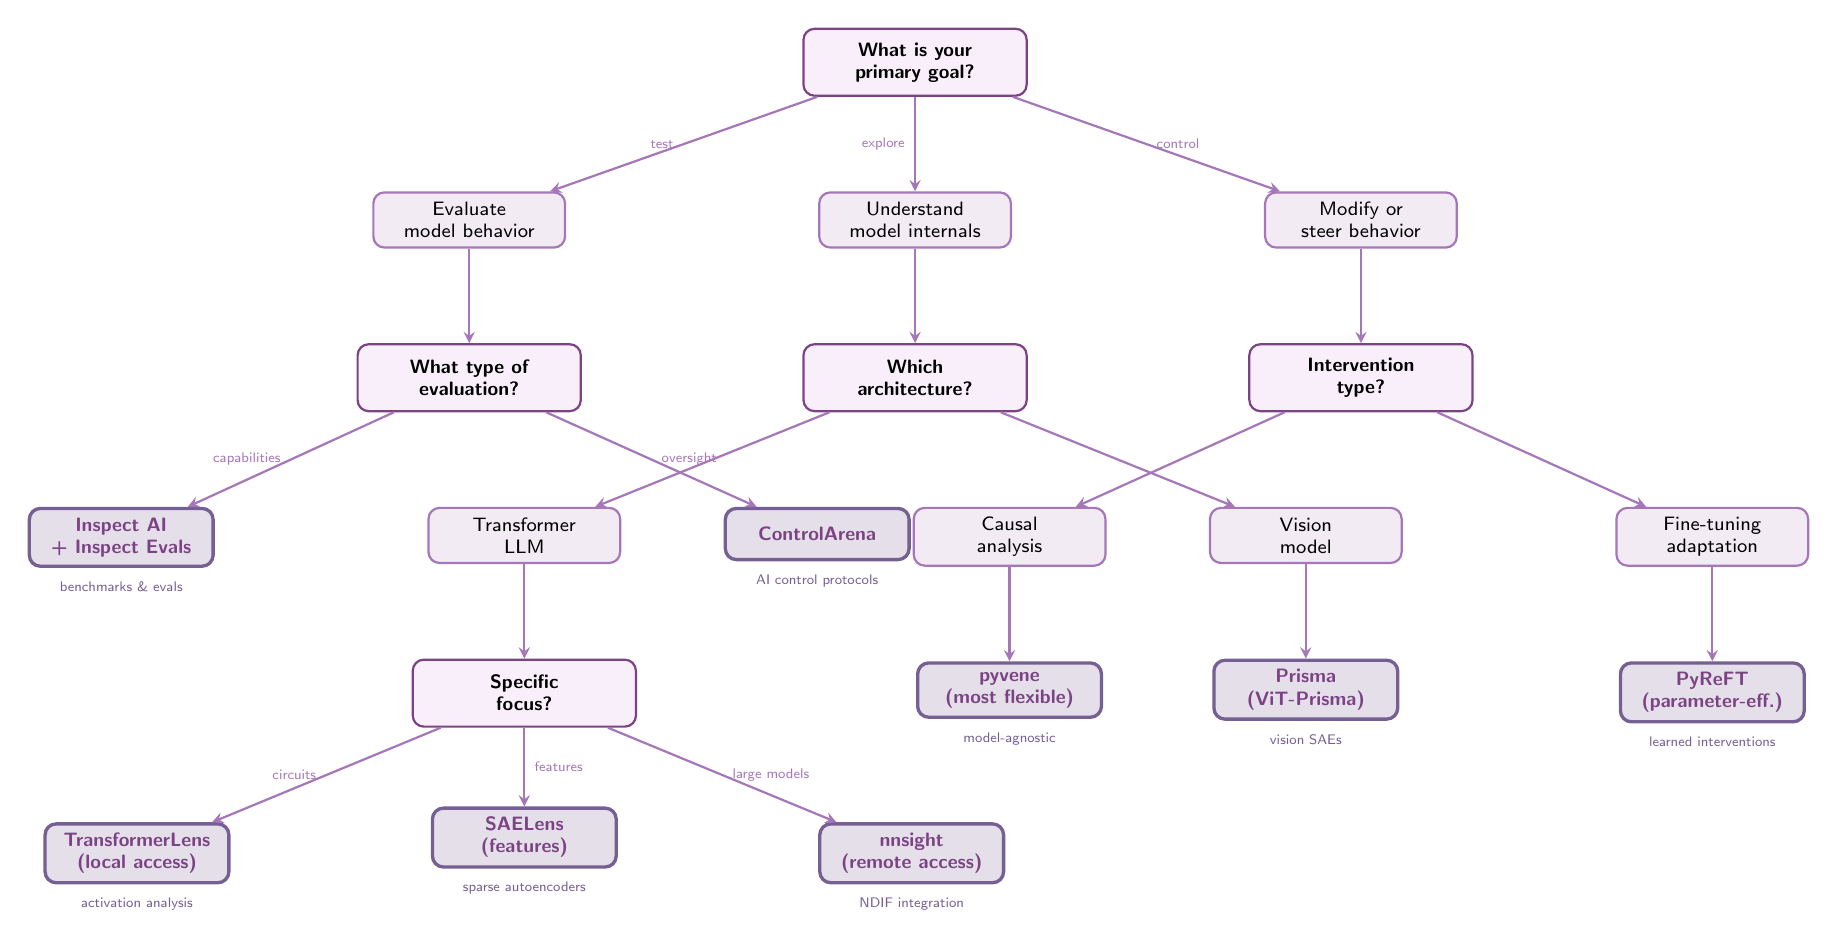
\begin{tikzpicture}[
    node distance=1.2cm and 1.5cm,
    every node/.style={align=center},
    question/.style={rectangle, draw=primary, thick, fill=accent!20, rounded corners, minimum width=2.8cm, minimum height=0.85cm, text width=2.6cm, font=\scriptsize\bfseries},
    answer/.style={rectangle, draw=secondary, thick, fill=secondary!15, rounded corners, minimum width=2.4cm, minimum height=0.7cm, text width=2.2cm, font=\scriptsize},
    tool/.style={rectangle, draw=tertiary, very thick, fill=tertiary!20, rounded corners, minimum width=2.3cm, minimum height=0.65cm, text width=2.1cm, font=\scriptsize\bfseries\color{primary}},
    arrow/.style={->, >=stealth, thick, color=secondary}
]

% Start node
\node[question] (start) {What is your\\primary goal?};

% Level 1 - Main branches
\node[answer, below left=of start, xshift=-1.5cm] (eval) {Evaluate\\model behavior};
\node[answer, below=of start] (understand) {Understand\\model internals};
\node[answer, below right=of start, xshift=1.5cm] (intervene) {Modify or\\steer behavior};

% Evaluation branch
\node[question, below=of eval] (evaltype) {What type of\\evaluation?};
\node[tool, below left=of evaltype, xshift=-0.3cm] (inspect) {\textbf{Inspect AI}\\+ Inspect Evals};
\node[tool, below right=of evaltype, xshift=0.3cm] (control) {\textbf{ControlArena}};

% Understanding branch
\node[question, below=of understand] (archtype) {Which\\architecture?};
\node[answer, below left=of archtype, xshift=-0.8cm] (transformer) {Transformer\\LLM};
\node[answer, below right=of archtype, xshift=0.8cm] (vision) {Vision\\model};

% Transformer sub-branch
\node[question, below=of transformer] (transformergoal) {Specific\\focus?};
\node[tool, below left=of transformergoal, xshift=-0.8cm] (tlens) {\textbf{TransformerLens}\\(local access)};
\node[tool, below=of transformergoal, yshift=0.2cm] (sae) {\textbf{SAELens}\\(features)};
\node[tool, below right=of transformergoal, xshift=0.8cm] (nnsight) {\textbf{nnsight}\\(remote access)};

% Vision branch
\node[tool, below=of vision] (prisma) {\textbf{Prisma}\\(ViT-Prisma)};

% Intervention branch
\node[question, below=of intervene] (inttype) {Intervention\\type?};
\node[answer, below left=of inttype, xshift=-0.3cm] (causal) {Causal\\analysis};
\node[answer, below right=of inttype, xshift=0.3cm] (finetune) {Fine-tuning\\adaptation};

\node[tool, below=of causal] (pyvene) {\textbf{pyvene}\\(most flexible)};
\node[tool, below=of finetune] (pyreft) {\textbf{PyReFT}\\(parameter-eff.)};

% Arrows from start
\draw[arrow] (start) -- (eval) node[midway, left, font=\tiny] {test};
\draw[arrow] (start) -- (understand) node[midway, left, font=\tiny] {explore};
\draw[arrow] (start) -- (intervene) node[midway, right, font=\tiny] {control};

% Evaluation arrows
\draw[arrow] (eval) -- (evaltype);
\draw[arrow] (evaltype) -- (inspect) node[midway, left, font=\tiny] {capabilities};
\draw[arrow] (evaltype) -- (control) node[midway, right, font=\tiny] {oversight};

% Understanding arrows
\draw[arrow] (understand) -- (archtype);
\draw[arrow] (archtype) -- (transformer);
\draw[arrow] (archtype) -- (vision);
\draw[arrow] (transformer) -- (transformergoal);
\draw[arrow] (transformergoal) -- (tlens) node[midway, left, font=\tiny] {circuits};
\draw[arrow] (transformergoal) -- (sae) node[midway, right, font=\tiny] {features};
\draw[arrow] (transformergoal) -- (nnsight) node[midway, right, font=\tiny] {large models};
\draw[arrow] (vision) -- (prisma);

% Intervention arrows
\draw[arrow] (intervene) -- (inttype);
\draw[arrow] (inttype) -- (causal);
\draw[arrow] (inttype) -- (finetune);
\draw[arrow] (causal) -- (pyvene);
\draw[arrow] (finetune) -- (pyreft);

% Additional tool annotations
\node[font=\tiny, text=tertiary, below=0.05cm of inspect] {benchmarks \& evals};
\node[font=\tiny, text=tertiary, below=0.05cm of control] {AI control protocols};
\node[font=\tiny, text=tertiary, below=0.05cm of tlens] {activation analysis};
\node[font=\tiny, text=tertiary, below=0.05cm of sae] {sparse autoencoders};
\node[font=\tiny, text=tertiary, below=0.05cm of nnsight] {NDIF integration};
\node[font=\tiny, text=tertiary, below=0.05cm of prisma] {vision SAEs};
\node[font=\tiny, text=tertiary, below=0.05cm of pyvene] {model-agnostic};
\node[font=\tiny, text=tertiary, below=0.05cm of pyreft] {learned interventions};

\end{tikzpicture}%
}
\caption{Decision tree for selecting AI safety and interpretability tools based on research objectives. Start at the top node and follow branches corresponding to your primary goal and constraints.}
\end{figure}

\textbf{Visualization and Auxiliary Tools:} Regardless of your primary path, several tools support any workflow. Use \textbf{CircuitsVis} for creating interactive visualizations of activations and attention patterns. \textbf{Neuronpedia} provides a web-based platform for exploring pre-computed SAE features and sharing interpretability findings. \textbf{Transformer Debugger} offers an interactive GUI for rapid exploration when working with small models like GPT-2.

\section{Community Resources}

Beyond individual tools, the AI safety and interpretability community maintains several valuable resources. The AI Safety Support website at \url{https://www.aisafety.com/projects} provides a community-maintained list of volunteer AI safety projects and tools. Anthropic's Transformer Circuits Thread at \url{https://transformer-circuits.pub/} offers an ongoing research publication series on mechanistic interpretability, including landmark work on induction heads, monosemanticity, and circuit tracing. The Open Source Mechanistic Interpretability Slack hosts an active community for tool development and research collaboration, while the LessWrong AI Alignment Forum facilitates community discussion and research sharing, including extensive coverage under the Sparse Autoencoders tag for SAE research.

\bibliographystyle{plainnat}
\bibliography{lecture}

\end{document}
